% !TEX program = xelatex

% {{{
\documentclass[14pt, a4paper]{extreport}
\usepackage[table, dvipsnames]{xcolor}


% force figure position
% \renewcommand{\textfraction}{0.05} 


% conditional formatting tables

% \definecolor{red}{rgb}{1,0,0}
\definecolor{blue}{rgb}{0,0.3,1}

\usepackage{tikz}
\usetikzlibrary{arrows.meta, positioning}

\usepackage{collcell}
\usepackage{pgf}

 %The min, mid and max values
\newcommand*{\MinNumber}{-0.3}%
\newcommand*{\MidNumber}{0.0} %
\newcommand*{\MaxNumber}{0.3}%

% \newcommand{\ApplyGradient}[1]{%
%   \ifdim #1 pt > \MidNumber pt
%     \pgfmathsetmacro{\PercentColor}{max(min(100.0*(#1 - \MidNumber)/(\MaxNumber-\MidNumber),100.0),0.00)} %
%     \edef\x{\noexpand\cellcolor{gray!\PercentColor}}\x\textcolor{black}{#1}%
%   \else
%     \pgfmathsetmacro{\PercentColor}{max(min(100.0*(\MidNumber - #1)/(\MidNumber-\MinNumber),100.0),0.00)} %
%     \edef\x{\noexpand\cellcolor{black!\PercentColor}}\x\textcolor{black}{#1}%
%   \fi
% }

\newcommand{\ApplyGradient}[1]{%
  \pgfmathsetmacro{\PercentColor}{100.0-max(min(100.0*(#1-\MinNumber)/(\MaxNumber-\MinNumber), 100.0), 0.00)}%
  \edef\x{\noexpand}\x\textcolor{black!\PercentColor}{#1}%
}

\newcolumntype{R}{>{\collectcell\ApplyGradient}l<{\endcollectcell}}
% \renewcommand{\arraystretch}{0}
% \setlength{\fboxsep}{3mm} % box size
% \setlength{\tabcolsep}{0pt}






\usepackage{fontspec}
\setmonofont{Iosevka Custom}

\usepackage{xcolor}

\usepackage{Alegreya}
\hyphenchar\font=-1

\renewcommand{\baselinestretch}{1.5}

\usepackage[left=30mm, top=20mm, right=10mm, bottom=20mm]{geometry}
\setlength\parindent{1.25cm}

\usepackage{indentfirst}

% word spacing

\sloppy
% \fontdimen2\font=0.3em % base word spacing
% \fontdimen3\font=2em % base word stretch
\fontdimen4\font=0em % base word squeeze


% toc

\usepackage{tocloft}

\setcounter{tocdepth}{3}

\setlength{\cftbeforetoctitleskip}{0pt} % remove extra margin from toc
\setlength{\cftaftertoctitleskip}{0pt} % remove extra margin from toc

\renewcommand{\thechapter}{} % remove numbering from chapters
\renewcommand\thesection{\arabic{section}} % reset numbering of sections to remove the leading dot

% indents in toc \cftsetindents{kind}{indent}{numwidth}
\cftsetindents{chapter}{0em}{0em}
\cftsetindents{section}{0em}{4mm}
\cftsetindents{subsection}{1em}{8mm}
\cftsetindents{subsubsection}{2em}{12mm}

% titles

\usepackage{titlesec}

\setcounter{secnumdepth}{3}

% indents in titles
\titlespacing{\chapter}{0pt}{0em}{1em}
\titlespacing{\section}{1.25cm}{2em}{1em}
\titlespacing{\subsection}{1.25cm}{2em}{1em}
\titlespacing{\subsubsection}{1.25cm}{2em}{1em}
\titlespacing{\paragraph}{1.25cm}{1em}{1em}

\newlength\titleindent
\setlength\titleindent{1.25cm}

\titleformat{\chapter}
  {\Large\center\bfseries\MakeUppercase}{}{0em}{}[]
\titleformat{\section}
  {\large}{\parbox[b]{4mm}{\bfseries\thesection\hfill}}{0em}{\bfseries}
\titleformat{\subsection}
  {\normalsize}{\parbox[b]{8mm}{\bfseries\thesubsection}}{0em}{\bfseries}
\titleformat{\subsubsection}
  {\normalsize}{\parbox[b]{12mm}{\bfseries\thesubsubsection}}{0em}{\bfseries}
\titleformat{\paragraph}
  {\normalsize}{\parbox[b]{12mm}{\bfseries}}{0em}{\bfseries}


% sources

\definecolor{mylinkcolor}{HTML}{0c7dbb}

\usepackage[colorlinks=true, citecolor=mylinkcolor]{hyperref}

\hypersetup{%
  colorlinks = true,
  linkcolor  = black
}


\usepackage[
    backend=biber,
    sorting=nyt,
    ibidtracker=false, % removes "там же"
    hyperref=true,
    bibstyle=gost-numeric,
    citestyle=authoryear
]{biblatex}

\addbibresource{sources.bib}

% }}}
\DeclareCiteCommand{\parencite}{\usebibmacro{prenote}}{\usebibmacro{citeindex}\normalsize{[}\printtext[bibhyperref]{\usebibmacro{cite}{\usebibmacro{postnote}}}}\normalsize{]}
% {{{
% img

\usepackage{graphicx}
\graphicspath{ {./img/} }

% codeblocks

\usepackage{listings}

\definecolor{backcolour}{rgb}{0.96,0.96,0.96}

\lstdefinestyle{mystyle}{
    backgroundcolor=\color{backcolour},
    basicstyle=\ttfamily\small,
%     breakatwhitespace=false,         
    breaklines=true,
%     captionpos=b,                    
%     keepspaces=true,                 
    % numbers=left,
    % numbersep=10pt,
%     showspaces=false,                
%     showstringspaces=false,
%     showtabs=false,                  
    tabsize=2,
    framexleftmargin=5pt,
    framexrightmargin=5pt,
    framextopmargin=5pt,
    framexbottommargin=5pt,
    frame=tb,
    framerule=0mm,
    aboveskip=1em,
    belowskip=1em,
}

\lstset{style=mystyle}

%{\multicitedelim}


% gloss

\usepackage{gb4e}


\makeatletter
% Definition of \ttfamily from latex.ltx
\DeclareRobustCommand\ttfamily
        {\not@math@alphabet\ttfamily\mathtt
         \fontfamily\ttdefault\small\selectfont}
\makeatother

% DOCUMENT

\begin{document}

\sloppy
\fontdimen2\font=0.3em % base word spacing
\fontdimen3\font=2em % base word stretch
\fontdimen4\font=0em % base word squeeze

\begin{titlepage}
  \newgeometry{left=20mm, top=20mm, right=20mm, bottom=20mm}
  \begin{center}
    tomo suli pi kama sona

    NIMI PI TOMO NI

    \vfill

    \textbf{tsbohc}

    \large
    \textbf{TOKI PONA: DATA-DRIVEN VOCABULARY ANALYSIS}

    \normalsize

    (tenpo ni la, lipu ni li pona ala) 

    \bigskip


    \vfill
    ma pona 2022

  \end{center}
\end{titlepage}

\setcounter{page}{2}
\restoregeometry

\renewcommand{\contentsname}{\let\clearpage\relax\chapter*{Contents}} % chapter* doesn't appear in toc
\tableofcontents

% }}}

% TODO: you know what would be cool? a sample density graph that shows how much corpus I have per year.

% ---

\chapter{Introduction}

% TODO: citation on relative speaker count
Toki Pona is the second most spoken constructed language in the world. Its core vocabulary consists of only 120-140 words, not including words that are rare and/or considered non-standard by the majority of speakers. Despite the small vocabulary size, Toki Pona can be effectively used to convey a wide range of ideas of varying complexity.

This research aims to perform the semantic analysis and classification of the vocabulary of Toki Pona.

Numerous dictionaries of Toki Pona exist, but only the most immediate word definitions are provided. They may be enough for someone learning the language to grasp the general idea, but are insufficient to reflect the way the words are used in all of their shades of meaning. Because of this, the said analysis cannot be performed without studying how the language is spoken.

One approach to solving this problem would be to develop a system of evaluating the speaker proficiency. The evaluated speakers of the language who passed the test can then be recruited. By the way of discussion every word can then be described in detail.

The primary difficulty of this approach is that the system which would evaluate speakers has to be created by the proficient speakers. In other words, this is a causality dilemma. This approach would also rely on the judgement of a relatively small sample of the community. With this approach, the results would be based on the perception of the usage patterns of the language and not the usage of the language itself.

% Natural languages do not experience this as severely. Natural languages have much longer histories, much closer ties in local culture, and much larger vocabularies. Because of this, are not as volatile as constructed languages.

A different approach is to let the data drive the analysis. An adequately large corpus can be compiled by a single person. Modern approaches to Natural Language Processing can then be used to obtain the data on the language change and the semantic distribution of the vocabulary. Observations made on this data can then serve as the basis for the semantic analysis of the vocabulary.

\begin{itemize}
  \item \textbf{Subject.} Semantic analysis and classification of vocabulary.
  \item \textbf{Object.} Toki Pona, a constructed language.
  \item \textbf{Goal.} Perform the semantic analysis and classification of the vocabulary of the language.
  \begin{itemize}
    \item \textbf{Problem.} Vocabulary cannot be analysed based on the existing resources as they do not contain sufficient information for analysis.
    \item \textbf{Solution.} Use natural language processing techniques to construct a semantic model of the language and base the analysis on it.
  \end{itemize}
  \item \textbf{Methodology.} Distributional semantics and natural language processing, namely language modelling (word embedding).
\end{itemize}


\paragraph{Objectives}

\begin{enumerate}
  \item Define and classify constructed languages.
  \item Describe toki pona, its philosophy, history, and unique features.
  \item Define distributional semantics.
  \item Define modern approaches to Natural Language Processing applicable to the research.
  \item Obtain the necessary corpora.
  \item Construct a vector space model of the language.
  \item Make observations on the model.
  \item Classify the vocabulary based on the observed semantic relationships between the words of the vocabulary.
\end{enumerate}


\paragraph{Relevance}

With the rise of the internet, constructed languages now have a place where they can live and thrive. Constructed languages are rapidly gaining popularity. Despite this, the only constructed language that has seen much representation in scientific writing is Esperanto.

The existing dictionaries of Toki Pona can greatly benefit from the findings of this research. This data can also be used as an aid in teaching the language to new speakers.

The Vector Space Model of Toki Pona constructed in the course of this research can find further use in information retrieval, topic modelling, text prediction, sentiment analysis, and many other areas.


\chapter{Distributional semantics and~constructed~languages}

\section{Natural language processing}
% {{{
``Linguistics is concerned not only with language per se, but must also deal with how humans model the world. The study of semantics, for example, must relate language expressions to their meanings, which reside in the mental models possessed by humans. <...> Whereas computational linguistics, as a subfield of linguistics, is concerned with the formal or computational description of rules that languages follow'' \parencite{nlpandcl}.

The aim of this research is to bridge the gap between the two disciplines, to use computational linguistics to build a semantic model of a constructed language. This model can then be used to explore the nuances of how humans speak the said language.

In turn, ``Natural Language Processing is a field at the intersection of computer science, artificial intelligence, and linguistics'' \parencite[7]{practicalnlp}. ``Natural language processing includes a range of algorithms, tasks, and problems that take human-produced text as an input and produce some useful information, such as labels, semantic representations, and so on, as an output'' \parencite[4]{realworldnlp}.

\begin{figure}[ht]
\bigskip
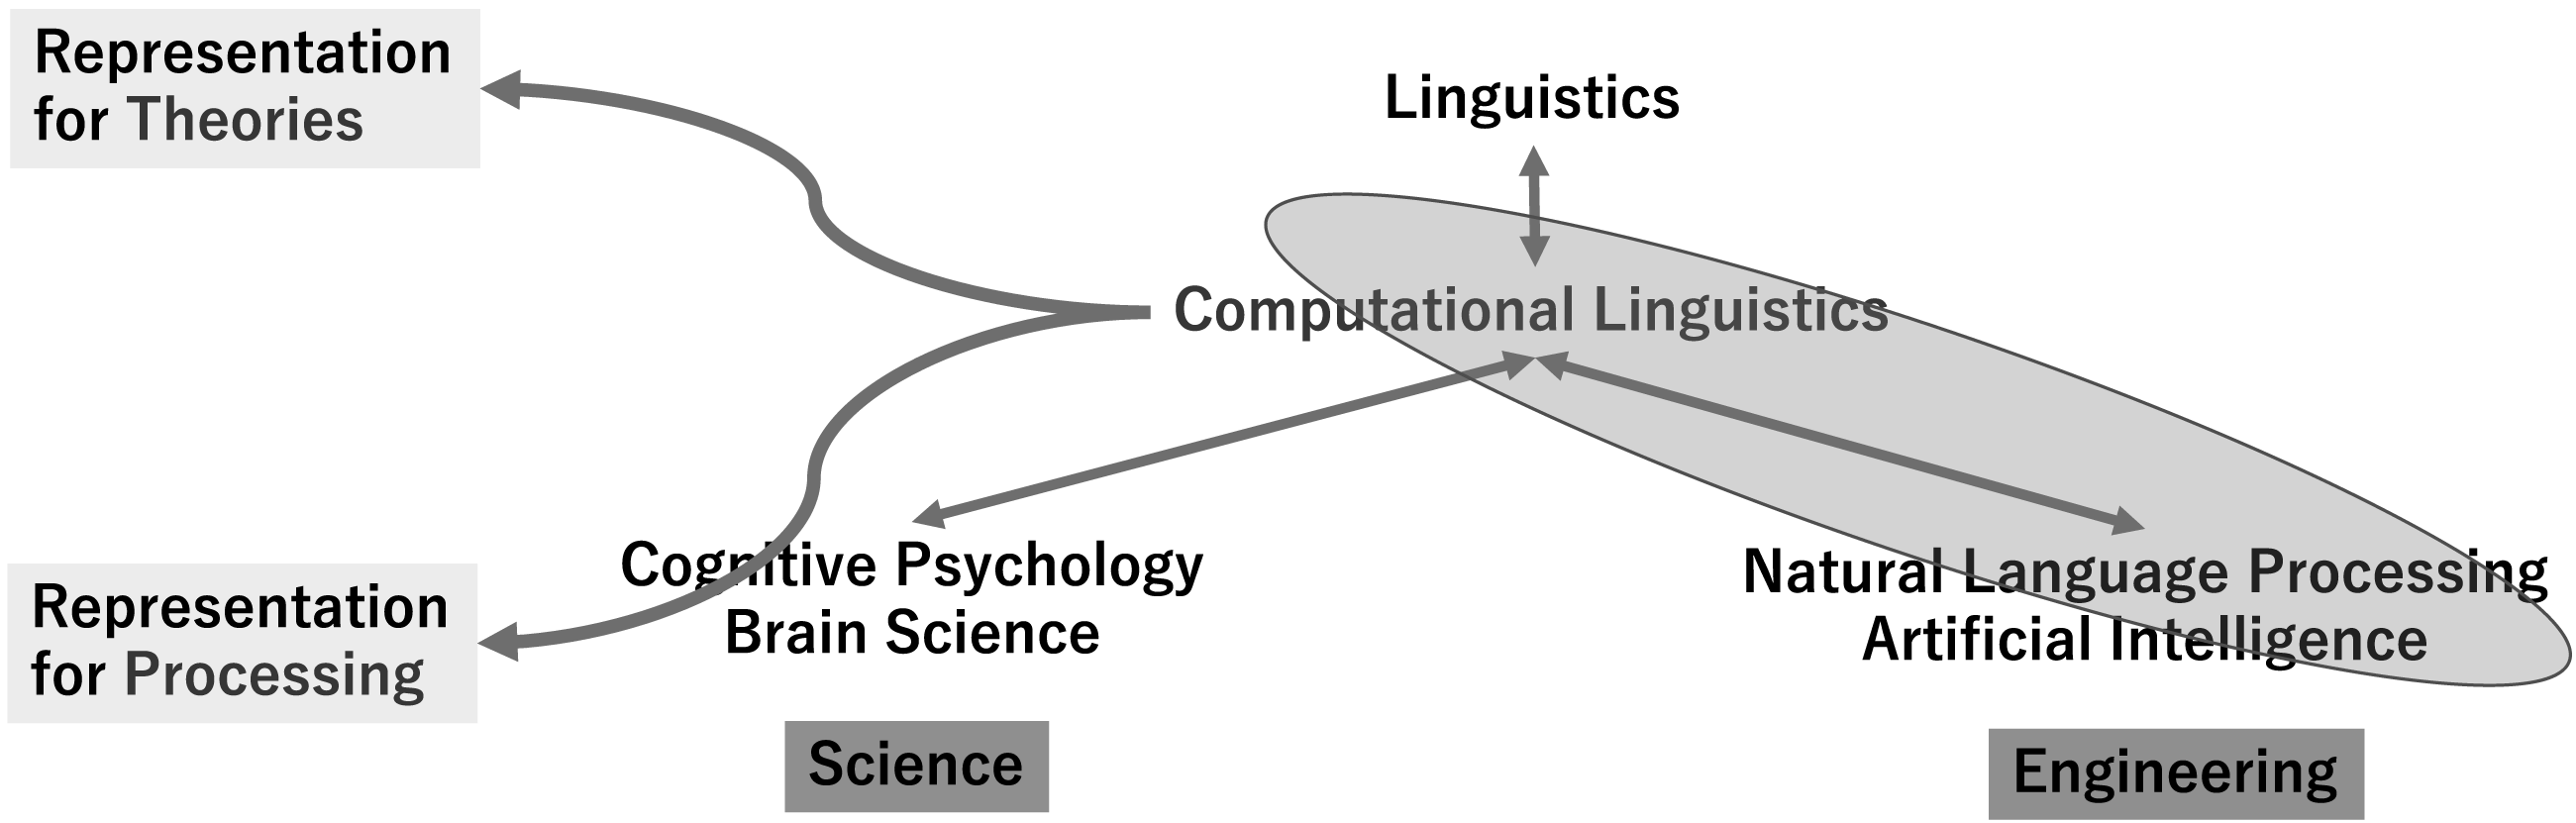
\includegraphics[width=14cm]{nlpcl}
\centering
\caption{Language-related disciplines \parencite{nlpandcl}}
\end{figure}
% }}}

\section{Distributional semantics}
% {{{
The core idea behind distributional semantics has roots in American structuralism (Harris) and British lexicology (Firth) and is known as the distributional hypothesis. In its simplest form, it states that ``similarity in meaning results in similarity of linguistic distribution'' \parencite{harris}.

The reverse of this statement is also true. That is, meaning can be inferred from context. The aim of distributional semantics is exactly that, to learn the meanings of linguistics units from a corpus of text. That is, distributional semantics can be described as the field that reverse-engineers the distributional hypothesis.

Distributional semantics was popularised by Firth in the 1950s. In a 1957 publication he wrote, ``the placing of a text as a constituent in a context of situation contributes to the statement of meaning since situations are set up to recognise use. <...> You shall know a word by the company it keeps!'' \parencite[11]{firth}.

The ideas introduced by the distributional hypothesis have received attention in cognitive science \parencite{mcdonald} and language learning \parencite{yarlett}.% }}}

\paragraph{Overview}
% {{{
Distributional semantics has become widespread with the adoption of information technology in the field of linguistic research.

Distributional semantics are most frequently applied by taking large amounts of text as input and pushing it through an abstraction algorithm to produce a distributional model as output.

\begin{figure}[ht]% {{{
  \bigskip
  \begin{tikzpicture}[>={Classical TikZ Rightarrow[]}]
    \node[text width=6cm] at (0,11.5) {Planets of the solar system are orbiting the \textit{sun}. The \textit{moon} is orbiting the earth. It's his antique \textit{typewriter} clacking. <...>};
    \draw[line width=1pt, ->] (4.5,11.5) -- (5.5,11.5) node[pos=0.5,below=0.5cm]{algorithm};
    \node [shape=rectangle] at (10,11.5) {
      \ttfamily
      \begin{tabular}{|lcc|}
        \hline
        & dim1    & dim2    \\
        \hline
        sun      & 0.11023 & 0.53848 \\
        % \textbf{seli}    & 0.172305 & 0.824956 \\
        moon     & 0.21575 & 0.44034 \\
        % \textbf{lete}    & 0.280345 & 0.881492 \\
        typewriter & 0.52834 & 0.05389 \\
        % \textbf{mu}      & 0.370184 & 0.188725 \\
        \hline
      \end{tabular}
    };

    \draw[->, line width=1](0,0) -- (0,8) node[pos=0.58,rotate=90,left=1.5cm]{dim1};
    \draw[->, line width=1](0,0) -- (8,0) node[pos=0.5,below=1cm]{dim2};

    \foreach \x in {0,0.2,0.4,0.6}
        \draw (\x*10 cm,1pt) -- (\x*10 cm,-3pt)
            node[anchor=north] {$\x$};

    \foreach \y in {0,0.2,0.4,0.6}
        \draw (1pt,\y*10 cm) -- (-3pt,\y*10 cm)
            node[anchor=east] {$\y$};

    \draw[lightgray] (0, 0) grid[xstep=1, ystep=1] (8, 8);
    \foreach \Point/\PointLabel in {(1.1,5.3)/sun, (2.1,4.4)/{moon  (0.21575, 0.44034)}, (5.2, 0.5)/typewriter}
 % (6.7,1.2)/mu,
% (2.1,3.9)/mun, (2.8,4.8)/lete, (3.4, 6.8)/sewi, 
    \draw[draw=gray,fill=gray] \Point circle (0.08) node[above right] {$\PointLabel$};

    \node[draw, text width=10cm, fill=white] at (8, 2.5) {
      \ttfamily
      cosine\_similarity(sun, moon) = 0.9711
      cosine\_similarity(sun, typewriter) = 0.2959
    };

  \end{tikzpicture}
  \centering
  \caption{Distributional semantics, an illustrated overview}
\end{figure}% }}}

In the model, the semantic representations are stored in the form of vectors. Vectors are essentially lists of numbers that refer to points in a multi-dimensional space. These vectors are referred to as word vectors.

The position of a word in the semantic space is determined by the values in its word vectors, that is, the context the word is most commonly used in. This way, words that are often used together are placed close to each other. The distance between points is a measurement of semantic similarity between the words they represent.

The multi-dimensionality of the word vector encodings can be reduced to only two or three dimensions. The resulting dimensions can then be used to create a projection of the model which can be observed by the human eye.

All of the approaches to distributional semantics share the quality of learning semantic representations from a corpus in an unsupervised manner. With a sufficiently large corpus, this excludes any but the collective human modelling of the world from the data.
% }}}

\subsection{Word vectors}
% {{{
``Word vectors represent words as multidimensional continuous floating point numbers where semantically similar words are mapped to proximate points in geometric space'' \parencite{ahireintro}.

In simpler terms, a word vector is a numerical representation of a word in a corpus relative to every other word in that corpus.

``Word vectors are numerical vector representations of word semantics, or meaning, including literal and implied meaning, meaning that word vectors can capture the connotation of words. And they combine all that into a dense vector (no zeros) of floating point values. This dense vector enables queries and logical reasoning'' \parencite[182]{lane2019natural}.

Essentially, word vectors are the means by which the aforementioned semantic distribution of words can be represented numerically. That is, a representation that is easy for a computer to understand and operate on.
% }}}

\subsubsection{Measuring semantic similarity}
% {{{
The semantic similary between two vectors is primary measured in two ways: using cosine similarity or euclidian distance.

The primary advantage of using one of these two methods is that they can be calculated for vectors of any dimensionality.

\paragraph{Euclidean distance}

The Euclidean distance between two points is the length of a line segment between the two points. It can also be defined as the shortest distance between two points in an n-dimensional space. For the purposes of calculating the Euclidean distance, the vectors are viewed as point coordinates.

\medskip
\[d_{Euc}(p, q) = \sqrt{\displaystyle\sum_{i=1}^{n} (p_i - q_i)^2} = \sqrt{(p_1 - q_1)^2 + (p_2 - q_2)^2 + ... + (p_n - q_n)^2}\]

\paragraph{Cosine similarity}

Cosine similarity is a measurement of similarity between two sequences of numbers. When calculating cosine similarity, the two sequences of numbers are viewed as vectors. Cosine similarity is equal the cosine of the angle between two vectors, that is, the dot product of the vectors devided by the product of their lengths.

Cosine similarity always falls into the interval \([-1, 1]\). Two parallel vectors have 
a cosine similarity of \(1\), two orthogonal (perpendicular to each other) vectors have a cosine similarity of \(0\), while two opposite vectors have a cosine similarity of \(-1\).

\medskip
\[s_{cos}(A, B) := cos(\th) = \frac {A \cdot B}{||A|| \cdot ||B||} = \frac {\displaystyle\sum_{i=1}^{n} A_i B_i}{\sqrt{\displaystyle\sum_{i=1}^{n} A_i^2} \sqrt{\displaystyle\sum_{i=1}^{n} B_i^2}}\]
\medskip

This method was chosen to simplify the process of comparing similarities between vector pairs. Where the Euclidean distance provides an absolute value, the cosine similarity provids a fraction.

% }}}

\subsection{Implementations}

One of the earliest implementations featured a simple counting algorithm. For each word in a corpus, the frequencies of each of the context words were counted. The counts were then normalised by the total number of collected word relationships \parencite{erkkatrin}.


% The principles of linear algebra can be applied to operate on word vectors and determine the degrees of similarity between them.

\subsection{Word vectors}

``Word vectors represent words as multidimensional continuous floating point numbers where semantically similar words are mapped to proximate points in geometric space'' \parencite{ahireintro}.

In simpler terms, a word vector is a numerical representation of a word in a corpus relative to every other word in that corpus.

``Word vectors are numerical vector representations of word semantics, or meaning, including literal and implied meaning. So word vectors can capture the connotation of words, like \textit{peopleness,} \textit{animalness,} \textit{placeness,} \textit{thingness,} and even \textit{conceptness.} And they combine all that into a dense vector (no zeros) of floating point values. This dense vector enables queries and logical reasoning'' \parencite[182]{lane2019natural}.

\paragraph{Word embedding}



% model dimensionality

% \subsection{Applications}
%
% The data produced via natural language processing has a variety of applications.

\section{Constructed languages}

\subsection{The notion of a constructed language}

\subsection{Classification}


\chapter{Language modelling and Toki Pona}

\section{Toki Pona}

\subsection{History}

\subsection{Phonology}

\subsection{Grammar}

\subsection{Vocabulary}

\section{Vector space model}

\subsection{Corpus acquisition}

\subsection{Text normalisation}

\subsection{Model construction}

\subsection{Projection and visualisation}

\subsection{Observations}

% \paragraph{Polysemy}
%
% ``Related senses are called polysemous: for example, school can refer to a building or an institution. In contrast, homonymous senses are unrelated: for example, a school of fish. All of the above senses of school are also lexicalised – established uses that a speaker would have committed to memory, rather than inferring from context'' \parencite[4]{emerson}.
%
% Toki Pona is highly resistant to lexicalisation. Because the vocabulary contains a very small number of words, they are inherently context-dependent. Any word can be used in any suitable context.




\printbibliography[heading=bibintoc,title={References}]

\end{document}



























% \chapter{Introduction}
%
% % TODO: you know what would be cool? a sample density graph that shows how much corpus I have per year.
%
% % The main obstacle in the discussion of semantics in the context of a constructed language is its high degree volatility. Upon conception, the words are assigned meanings by the creator. As the language enters use, it develops patterns that fill the practical requirements of its speakers.
%
% %Such requirements may arise due to an oversight in the design, a desire to improve it, or to accomodate new realia.
%
% % In the case of Toki Pona, this includes numerous proposed number systems, new words that took some shade of meaning from existing words to make it easier to convey a certain idea.
%
% % Constructed languages do not have strong ties in culture, tradition, or geographical location. This causes the said languages to experience substantial changes much more rapidly than natural languages. Because of this, the discussion of semantics that relies on the original dictionary proposed by the creator is no longer sustainable. To perform analysis that reflects the current state of the vocabulary, the analysis has to be grounded in the current usage patterns of the language.
%
% % This poses a problem: how can usage patterns of a language be condensed into a form suitable for analysis?
%
%
% \chapter{Distributional semantics and constructed languages}
%
% \section{The notion of a constructed language}
%
% \subsection{Classification}
%
% \paragraph{Auxiliary}
% \paragraph{Philosophical}
% \paragraph{Artistic}
%
% % \section{Semantic metalanguage}
% % \subsection{Semantic decomposition}
%
% \section{Distributional semantics}
%
% \subsection{Distributional hypothesis}
%
% ``The placing of a text as a constituent in a context of situation contributes to the statement of meaning since situations are set up to recognise use. ... You shall know a word by the company it keeps!'' \parencite[11]{firth}.
%
% Distributional semantics is based on this hypothesis, ``which states that similarity in meaning results in similarity of linguistic distribution'' \parencite{harris}. This means that words that are semantically related, such as ``beer'' and ``whiskey'', are used in similar contexts: (he had too much <...>, the <...> made him drunk, a bottle of <...>).
%
% ``Distributional semantics reverse-engineers the process, and induces semantic representations from contexts of use'' \parencite{boleda}.
%
% \section{Natural language processing}
%
% ``Linguistics is concerned not only with language per se, but must also deal with how humans model the world. The study of semantics, for example, must relate language expressions to their meanings, which reside in the mental models possessed by humans. ... Whereas computational linguistics, as a subfield of linguistics, is concerned with the formal or computational description of rules that languages follow'' \parencite{nlpandcl}.
%
% The aim of this research is to bridge the gap between the two disciplines, to use computational linguistics to construct a model of a language. This model can then be used to explore the nuances of how humans speak the said language. That is, to gain insight into the semantics of the language.
%
% In turn, ``Natural Language Processing is a field at the intersection of computer science, artificial intelligence, and linguistics'' \parencite[7]{practicalnlp}. ``Natural language processing includes a range of algorithms, tasks, and problems that take human-produced text as an input and produce some useful information, such as labels, semantic representations, and so on, as an output'' \parencite[4]{realworldnlp}.
%
%
% \subsection{Word embedding}
%
% \subsubsection{Word vectors}
%
% ``Word vectors represent words as multidimensional continuous floating point numbers where semantically similar words are mapped to proximate points in geometric space'' \parencite{ahireintro}.
%
% In simpler terms, a word vector is a numerical representation of a word in a corpus relative to every other word in that corpus.
%
% ``Word vectors are numerical vector representations of word semantics, or meaning, including literal and implied meaning. So word vectors can capture the connotation of words, like \textit{peopleness,} \textit{animalness,} \textit{placeness,} \textit{thingness,} and even \textit{conceptness.} And they combine all that into a dense vector (no zeros) of floating point values. This dense vector enables queries and logical reasoning'' \parencite[182]{lane2019natural}.
%
% Essentially, word vectors are the means by which the aforementioned semantic distribution of words can be represented numerically. That is, a representation that is easy for a computer to understand and operate on.
%
% \subsubsection{Vector space model}
%
% % TODO
% ``In 2012, Thomas Mikolov, an intern at Microsoft, found a way to encode the meaning of words in a modest number of vector dimensions'' \parencite[184]{lane2019natural}. Later, this project received the name of Word2vec.
%
% ``Word2vec learns the meaning of words merely by processing a large corpus of unlabeled text. No one has to label the words in the Word2vec vocabulary. ... And no one has to tell Word2vec that soccer is a sport, or that a team is a group of people, or that cities are both places as well as communities. Word2vec can learn that and much more, all on its own! All you need is a corpus large enough to mention Marie Curie and Timbers and Portland near other words associated with science or soccer or cities'' \parencite[184]{lane2019natural}.
%
% The application of language modelling to the research of constructed languages possesses the benefit of providing data from which observations can be made. That is, semantic distinctions between individual words become apparent because of the context the words are used in, not because the creator associated a particular concept with a particular term.
%
% As an output, vector space models provide a collection of multidimensional vectors associated with lables, i.e. tokens.
%
% \paragraph{Visualisation}
%
% % \section{Zipf's law}
%
% \section{Summary}
%
%
% \chapter{Model construction and analysis}
%
% \section{Toki Pona}
%
% \subsection{History}
%
% % \subsection{Phonology}
% % \subsection{Vocabulary}
%
% \paragraph{Phonemic inventory}
%
% \begin{figure}[ht]
%   \begin{center}
%     \ttfamily
%     \begin{tabular}{|r|c|c|c|}
%       \hline
%       & Labial & Coronal & Dorsal \\
%       \hline
%       Nasal & m & n & \\
%       \hline
%       Stop & p & t & k \\
%       \hline
%       Fricative & & s & \\
%       \hline
%       Approximant & w & l & j \\
%       \hline
%     \end{tabular}
%   \end{center}
%   \caption{Consontants}
% \end{figure}
%
% \begin{figure}[ht]
%   \begin{center}
%     \ttfamily
%     \begin{tabular}{|r|c|c|}
%       \hline
%       & Front & Back \\
%       \hline
%       Close & i & u \\
%       \hline
%       Mid & e & o \\
%       \hline
%       Open & \multicolumn{2}{c|}{a} \\
%       \hline
%     \end{tabular}
%   \end{center}
%   \caption{Vowels}
% \end{figure}
%
% \paragraph{Syllables}
%
% % \section{Toolkit}
% % \paragraph{Python}
% % \paragraph{Nltk}
% % \paragraph{Panphon}
% % \paragraph{Word2vec}
% %
% % also gensim
% % (hmmm, could split the corpora into chunks based on direct object and verb markers and etc and extract n-grams from the result)
%
% \section{Corpora acquisition}
%
% % As was discussed previously, language modelling is highly dependent on corpora.
%
% \paragraph{Scraping}
%
% ``Web scraping is the practice of gathering data through any means other than a program interacting with an API (or, obviously, through a human using a web browser). This is most commonly accomplished by writing an automated program that queries a web server, requests data (usually in the form of HTML and other files that compose web pages), and then parses that data to extract needed information'' \parencite[10]{mitchell2015web}.
%
% For the purposes of this research, the r/tokipona subreddit (reddit.com/r/tokipona/) was scraped for text posts and comments via \parencite{pistocop}. 4419 text posts and 34043 comments were obtained. 46665 sentences were obtained from tatoeba.org via the downloads page.
%
% The data was compiled into a single CSV file. Each entry consists of an id, username, UTC timestamp, permalink, and body.
%
% % \begin{lstlisting}
% % ex3amx5,cr99am,soweli ni li pona li suwi ! sina pali ala pali e len soweli ni ? : ),1565982610,t3_cr99am,/r/tokipona/comments/cr99am/soweli_mi_toki_e_ni/ex3amx5/
% % ew14xvs,cj0w9g,"democracy, rule by the majority → *lawa li tan suli kulupu*",1565015252,t1_evbivw7,/r/tokipona/comments/cj0w9g/ideologies/ew14xvs/
% % ...
% % \end{lstlisting}
%
%
% % TODO: bytes table? or maybe later in model construction
%
% % TODO: provide examples how the data was transformed
%
% \paragraph{Normalisation}
%
% % TODO: definition of text normalisation
%
% Proper names were removed from the data, as they largely do not affect the general idea behind the sentence. For example,
%
% \begin{exe}
% \ex
% toki Nijon li pona kute tawa mi. toki li pona kute tawa mi.
% \glt I like how Japanese sounds. I like how the language sounds.
% \end{exe}
%
% Consecutive strings of tokens from the source text which are present in the dictionary were extracted into sentences. Toki Pona is not an inflected language, hence there is now need for lemmatisation. Any sentence whose length was less than 4 was discarded.
%
% Any punctuation symbols and formatting code was removed from the dataset. The resulting corpus consists of 84270 sentences, each with a timestamp.
%
%
% \section{Vector space model}
%
% \subsection{Model construction}
%
% The model was trained on the corpus described above.
%
% Word2vec was chosen over Fasttext as Word2vec has proved better suited for working with uninflected languages.
%
% \begin{figure}[ht]
% \bigskip
% 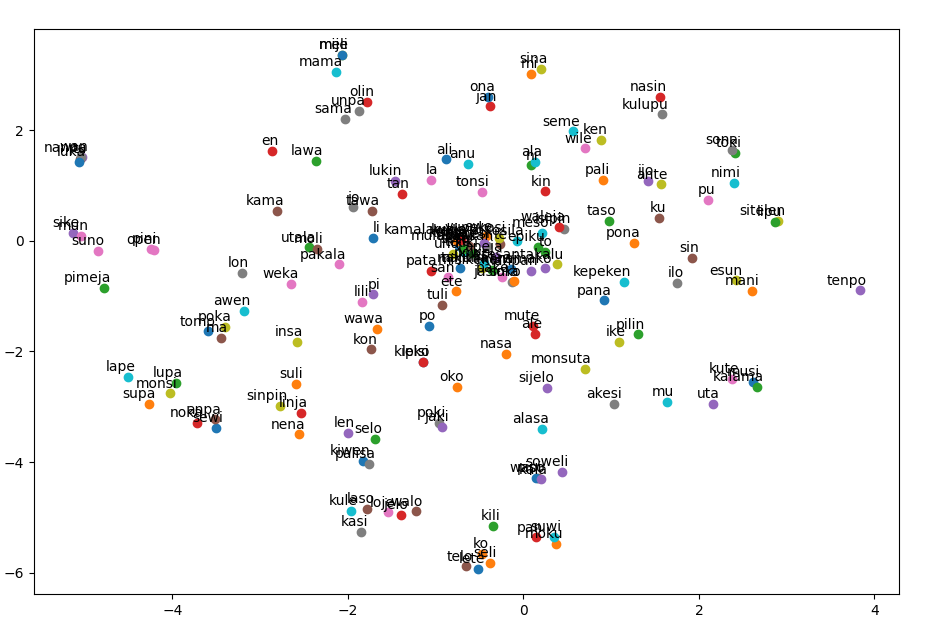
\includegraphics[width=.95\textwidth]{model}
% \centering
% \caption{Toki Pona Vector Space Model}
% \end{figure}
%
%
% \subsection{Semantic clustering}
%
% The model correctly groups semantically relevant words:
%
% \begin{itemize}
%   \item \textbf{Animals.} soweli (animal), waso (bird), kala (fish), alasa (hunt)
%   \item \textbf{Sound production and reception.} uta (mouth), kute (ear), kalama (sound), mu (onomatopoeia)
%   \item \textbf{Celestial bodies and time.} mun (moon), suno (sun), sike (circle), pimeja (black)
%   \item \textbf{Commerce.} esun (trade), mani (currency)
%   \item \textbf{Colours.} kule (color), jelo (yellow), loje (red), kasi (green), walo (white), etc.
%   \item \textbf{Writing.} sitelen (symbol), lipu (book), nimi (word), pu (the first official Toki Pona book)
%   \item \textbf{Relationships.} olin (love), unpa (sex), meli (female), mije (male), mama (parent), sama (same, occ. sibling)
%   \item \textbf{Pronouns.} mi (I), sina (II), ona (III), jan (person)
%   \item \textbf{Destruction.} utala (fight), pakala (break), moli (death)
%   \item \textbf{Location.} poka (beside), insa (inside), and weka (away), as well as anpa (below), noka (leg), sewi (above)
%   % \item \textbf{Sturdiness.} kiwen (small hard object), palisa (long hard object)
% \end{itemize}
%
% \paragraph{Observations}
%
% Sona (knowledge) and toki (language) were found to be semantically similar by the model. This is a testament to the fact that the two concepts often intersect in Toki Pona conversations, as a large portion of the community is interested in linguistics in one way or another.
%
% Pimeja (black) is disjointed from the rest of the colours due to its usage in the indication of time of day, e.g tenpo suno (daytime) and tenpo pimeja (nighttime).
%
%
%
% % \section{Zipf's law}
% % \section{N-grams}
%
% \section{Summary}
%
%
% \chapter{Conclusion}
%
% \printbibliography[heading=bibintoc,title={References}]
%
% \end{document}


% \begin{figure}[ht]
%   \bigskip
%   \begin{tikzpicture}[>={Classical TikZ Rightarrow[]}]
%     \node[text width=6cm] at (-5,0) {Planets of the solar system are orbiting the \textit{sun}. The \textit{moon} is orbiting the earth. It's his antique \textit{typewriter} clacking. <...>};
%     \draw[line width=1pt, ->] (-0.5,0) -- (0.5,0) node[pos=0.5,below=0.5cm]{algorithm};
%     \node [shape=rectangle] at (5,0) {
%       \ttfamily
%       \begin{tabular}{|lcc|}
%         \hline
%         & dim1    & dim2    \\
%         \hline
%         sun      & 0.11023 & 0.53848 \\
%         % \textbf{seli}    & 0.172305 & 0.824956 \\
%         moon     & 0.21575 & 0.44034 \\
%         % \textbf{lete}    & 0.280345 & 0.881492 \\
%         typewriter & 0.52834 & 0.05389 \\
%         % \textbf{mu}      & 0.370184 & 0.188725 \\
%         \hline
%       \end{tabular}
%     };
%   \end{tikzpicture}
%   \centering
%   \caption{Producing semantic representations from text}
% \end{figure}
